\section{Methodology}
\label{sec:-method}

\subsection{Challenges}
Several properties of the Tumblr network make a complex web crawler the 
only tool capable of extracting information from it effectively within 
the time frame of this project.  

Tumblr, unlike Twitter, does not assign unique numerical identifiers 
to its users.  Instead, users are referred to only by the plaintext URL 
that forms their identity.  This complex identifier makes the traversal 
of Tumblr over the namespace unfeasible.  Instead, user identification 
must rely upon encounters with those names in a corpus of data.

We construct a program to start with a single user seed, and proceed 
through all publicly available connections with that user, collecting 
additional usernames on which to repeat this process.  There are a 
number of API tools provided by Tumblr to make accessing its network 
via standalone applications possible.  Unfortunately, those tools were 
designed with a different set of functionality in mind.  The API 
client wrappers do not provide a complete enough set of data for the 
analyses we had in mind.  They do, however, provide a crucial subset 
that cannot be extracted via any other method.

The Tumblr API can be accessed through several different wrapper 
libraries.  Early in the project, we decided to use Python to create 
our Tumblr data collection mechanism.  Python was chosen for its 
low prototype-to-application turnaround time, its robust 
multiprocessing capabilities, and the perceived efficacy of the 
Python client library for the Tumblr API.  Unfortunately, the Python 
library abstracts away a great deal of important functionality, 
including a very brittle JSON-parsing system.  The library did not 
react well to the presence of Unicode characters within the API 
responses.  Unfortunately, Unicode characters are one of the primary 
means by which users customize the look and feel of their blogs and 
blog entries.

For this reason, the API wrapper was discarded in favor of direct 
access via HTTP.  This solved the Unicode corruption.  Unfortunately, 
the API was deficient in other areas.  It did not reliably distinguish 
between reblogs and original posts, it did not always return results 
that matched the specifications according to the documentation, it did 
not return well-formed data regarding notes and posts, and in the case 
of corrupt requests, it generally broke in interesting ways rather 
than predictable ones.

For these reasons, we supplemented access to the API with the actions 
of an HTML crawler over each user.  The differences in HTML generated 
by the user themes prevented reliable access to certain data points, 
but between the API responses and the HTML we were able to build a 
clear picture of user activity over the section of Tumblr we 
traversed.  The operation of the crawler we created is described 
in detail in the following subsection, and in Figure \ref{crawler}.

\subsection{Data Collection}

The crawler processes ran on a long-generic ACISS node with twelve 
cores, with 512 crawler instances pulling data from the network, 
and 200 database workers storing that data in a relational database.

\begin{figure}
  \begin{algorithmic}[1]
    \Require usernames initialized with a well-connected user
    \Procedure{Crawl}{$usernames,usersseen,dbQ$}
    \While{usernames not empty}
    \State $user.1 \gets usernames.pop$
    \State $blog \gets open(user.1)$
    \State $user.2 \gets blog.postCount$
    \State $user.3 \gets blog.lastActive$
    \State $dbQ.push(user)$ \Comment{send user to database worker}
    \ForAll{posts in blog}
    \If{post is reblogged}
    \If{source not in usersseen}
    \State $usersseen.push(post.source)$
    \State $usernames.push(post.source)$
    \EndIf
    \State $Continue$\Comment{Go to next post}
    \ElsIf {post is original}
    \State $postOut.1 \gets user.1$
    \State $postOut.2 \gets post.id$
    \State $postOut.3 \gets post.type$
    \State $postOut.4 \gets post.timestamp$
    \State $postOut.5 \gets post.notecount$    
    \State $dbQ.push(postOut)$
    \ForAll{notes on post}
    \State $noteOut.1 \gets note.source$
    \State $noteOut.2 \gets note.via$
    \State $noteOut.3 \gets post.id$
    \State $noteOut.4 \gets note.type$
    \State $dbQ.push(noteOut)$
    \If{note.source not in usersseen}
    \State $usersseen.push(note.source)$
    \State $usernames.push(note.source)$
    \EndIf
    \If{note.via not in usersseen}
    \State $usersseen.push(note.via)$
    \State $usernames.push(note.via)$
    \EndIf
    \EndFor
    \EndIf
    \EndFor
    \EndWhile
    \State \textbf{return} $True$    
    \EndProcedure
    \Procedure{databaseWork}{$dbQ$}
    \While{dbQ not empty}
    \State $database.write(dbQ.pop)$
    \EndWhile
    \EndProcedure
  \end{algorithmic}
%%% Local Variables: 
%%% mode: latex
%%% TeX-master: "main"
%%% End: 

  \caption{Crawler operation}\label{crawler}
\end{figure}

We have found that reblogs do not share the same post ID as the original 
post.  In order to avoid adding duplicate posts (and the shared notes 
associated with those posts) to the record, we defer the collection of 
reblogged posts, adding the origin of that post to the queue, to be 
crawled by a subsequent instance.  When the user that originally 
created the content is crawled, that post will contain reblog 
information linking that reblogging user, and the user from whom they 
reblogged the content.  Each reblog is therefore not only a 
relation between a user and a post, but potentially between three 
uses in total: User Alice who creates content, user Bob who reblogs 
that content from Alice, and use Charles who reblogs Alice's content 
via Bob.


These relationships are abstracted into records of users, notes, and pages, 
represented by tuples and passed to a managed queue in 
shared memory.  The database workers pull from this queue, and use 
the cardinality of the tuples to discern which table in the SQLite 
database should take the information.  Each database process 
maintains a separate database file on disc, in order to maximize 
speed-up from parallelization on filesystem writes.  Later, a 
separate program stitched the databases together for subsequent 
analysis.

\subsection{Data Storage and Analysis}
\begin{figure*}
\centering
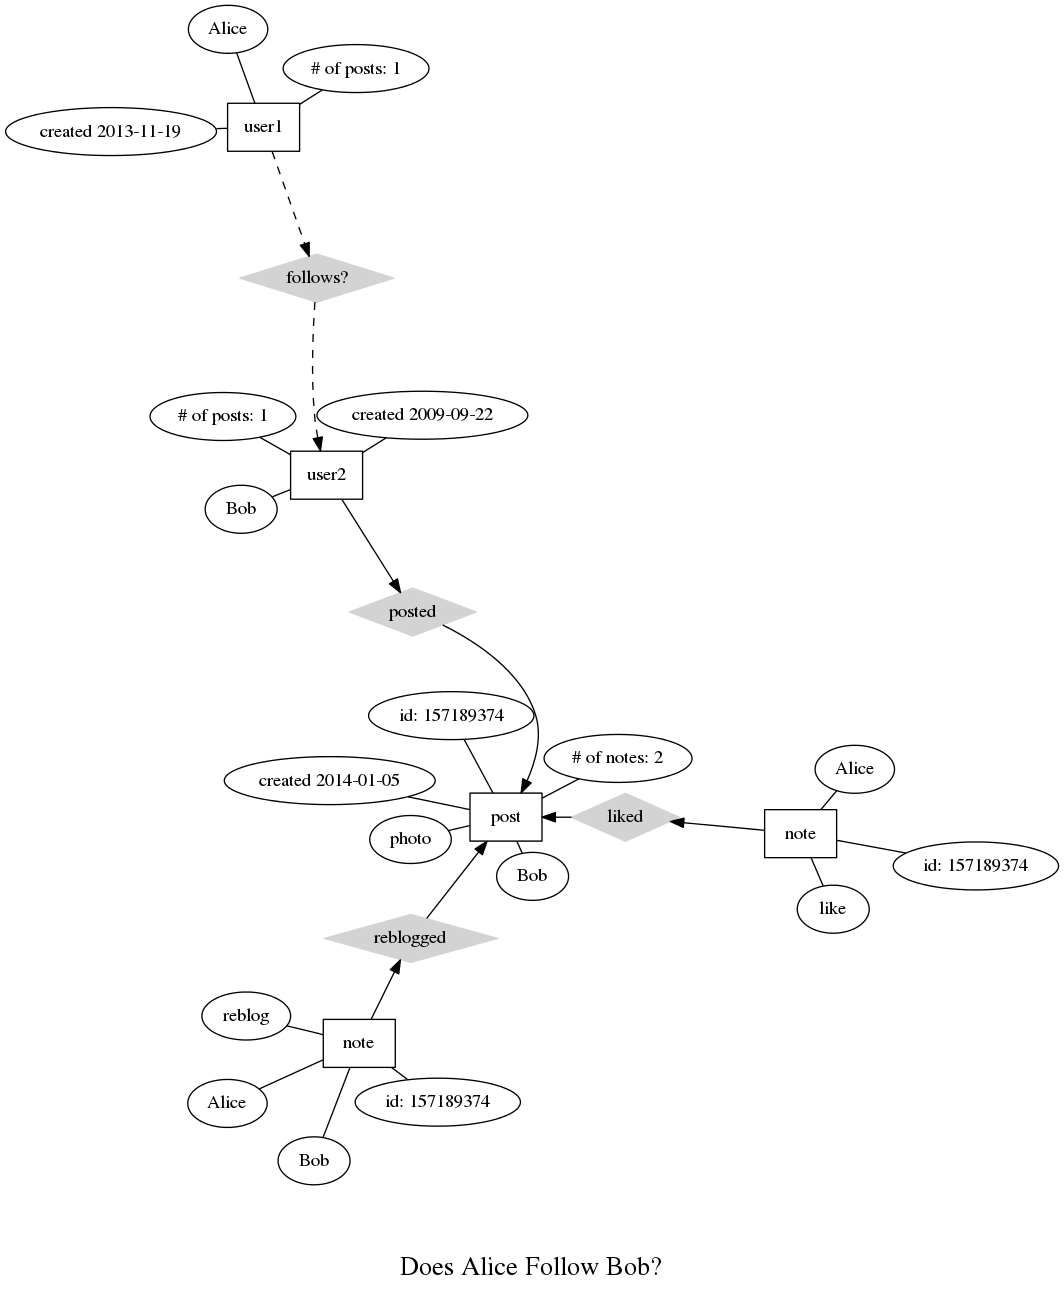
\includegraphics[width=\linewidth]{relations}
 \caption{Here we see a hypothetical relationship between two users}
 \label{fig:relations}
\end{figure*}
For each user, we logged their unique username, the number of posts 
they have contributed to Tumblr, and the date they joined. 
For each of those posts, we logged the unique post identifier, the 
date posted, the post type, and the number of notes.
For each of those notes, we log the username of the user who created 
the note, the username of the user they reblogged it from (blank if 
it's a like), the type, and the unique ID of the post this note is 
associated with.  While these records sum up the data nodes we have, 
the edges relating these nodes are only exposed upon analysis on this 
data set.  Of the many ways these data can be related, we examine only 
a fraction within the narrow time frame of this project.

While we only have access to explicit links between users and content, 
we speculate that these connections reflect the implicit connections 
between users.  The first hypothesis we ventured in the course of this 
research was that a collection of likes and reblogs concerning a pair 
of users, if carefully collected and isolated from external data, 
represent a ``user follows user'' relationship.  Specifically, if a 
user likes a statistically significant (compared to the activity level 
of that user) number of pieces of content published by another user, 
that may indicate that the first user follows the second.  In addition, 
if the first user has also reblogged content via that second user, this 
is another data point that, when taken together with the first, may 
suggest a following relationship.  By encoding these notions into a 
query over the database, we develop a prototypical method for 
identifying user followers, and show some samples from our application 
of that method to our dataset.


We also venture answers to some more conventional questions.  These, 
we answer using a multistage process.  First, we developed SQL queries 
and tested them against the small subsections of the database before 
deploying them onto the completely stitched-together database.  Some 
of the results from this stage were not yet in a form that is conducive 
to easy comprehension by humans.  To further process some of this data, 
we made use of a Python extension called NumPy, a tool designed to 
support the storage and analysis of very large sets of data.  Once 
this data had been reduced to a salient array of data points, we used 
gnuplot to generate the bar graphs seen later in the paper.


Firstly, and most simply, we would like to know what kind of post is 
most popular among users.  There are two ways to measure popularity: We 
could either monitor the prevalence of that type over all of the posts 
in our corpus of data, or we could monitor the note count over all such 
posts.  We have measured both separately, and present the results in the 
following section.

We would also like to know some things about the shape of the Tumblr 
network.  For this reason, we have analyzed the number of reblogs per 
user, and compared it to the number of original posts for those same 
users.  In addition, we present the number





There are several properties of the network that bear mentioning before 
we dive into the specifics of how to analyze our data.  Firstly, likes 
and reblogs are conserved across all instances of a post.  For likes, 
this means that a like on a reblog of content is indistinguishable from 
a like on the original piece of content itself.
%%% Local Variables: 
%%% mode: latex
%%% TeX-master: "main"
%%% End: 
